\chapter{Temporal Analysis of the Design and Development of Mobile Applications}
\label{ch:findings_chapter}
Sieveable enabled retrieving a sample of apps across multiple search criteria to meet a diverse set of search goals.
In this chapter, I present illustrative temporal analysis examples to understand how apps are evolved over time.

\section{Visual Design Mining}

Mobile UI design is always evolving and new guidelines are put into place to create a consistent experience across the platform.
For instance, Google introduced material design, a design language that makes use of elements from print design, responsive transitions, and depth effects \cite{Google_Material_Design}.
Google announced the main concepts of the design language on June 25, 2014.
Since then several third-party implementations have been introduced and used by developers.
A year later, Google introduced an official library called the Android Design Support Library, which allows developers to implement a number of material design components that are backward compatible with old devices.
We can use Sieveable to find apps that use specific material design components and find when they were adopted by developers.
We can also aggregate the results by download count and find trends in implementing them among popular and less popular apps.

\subsection{Material Design Components}
In this section, I present a set of analyses on the adoption rate of three major material design components over time.

\subsubsection{Floating Action Button}
\begin{figure}[H]
	\centering
	{{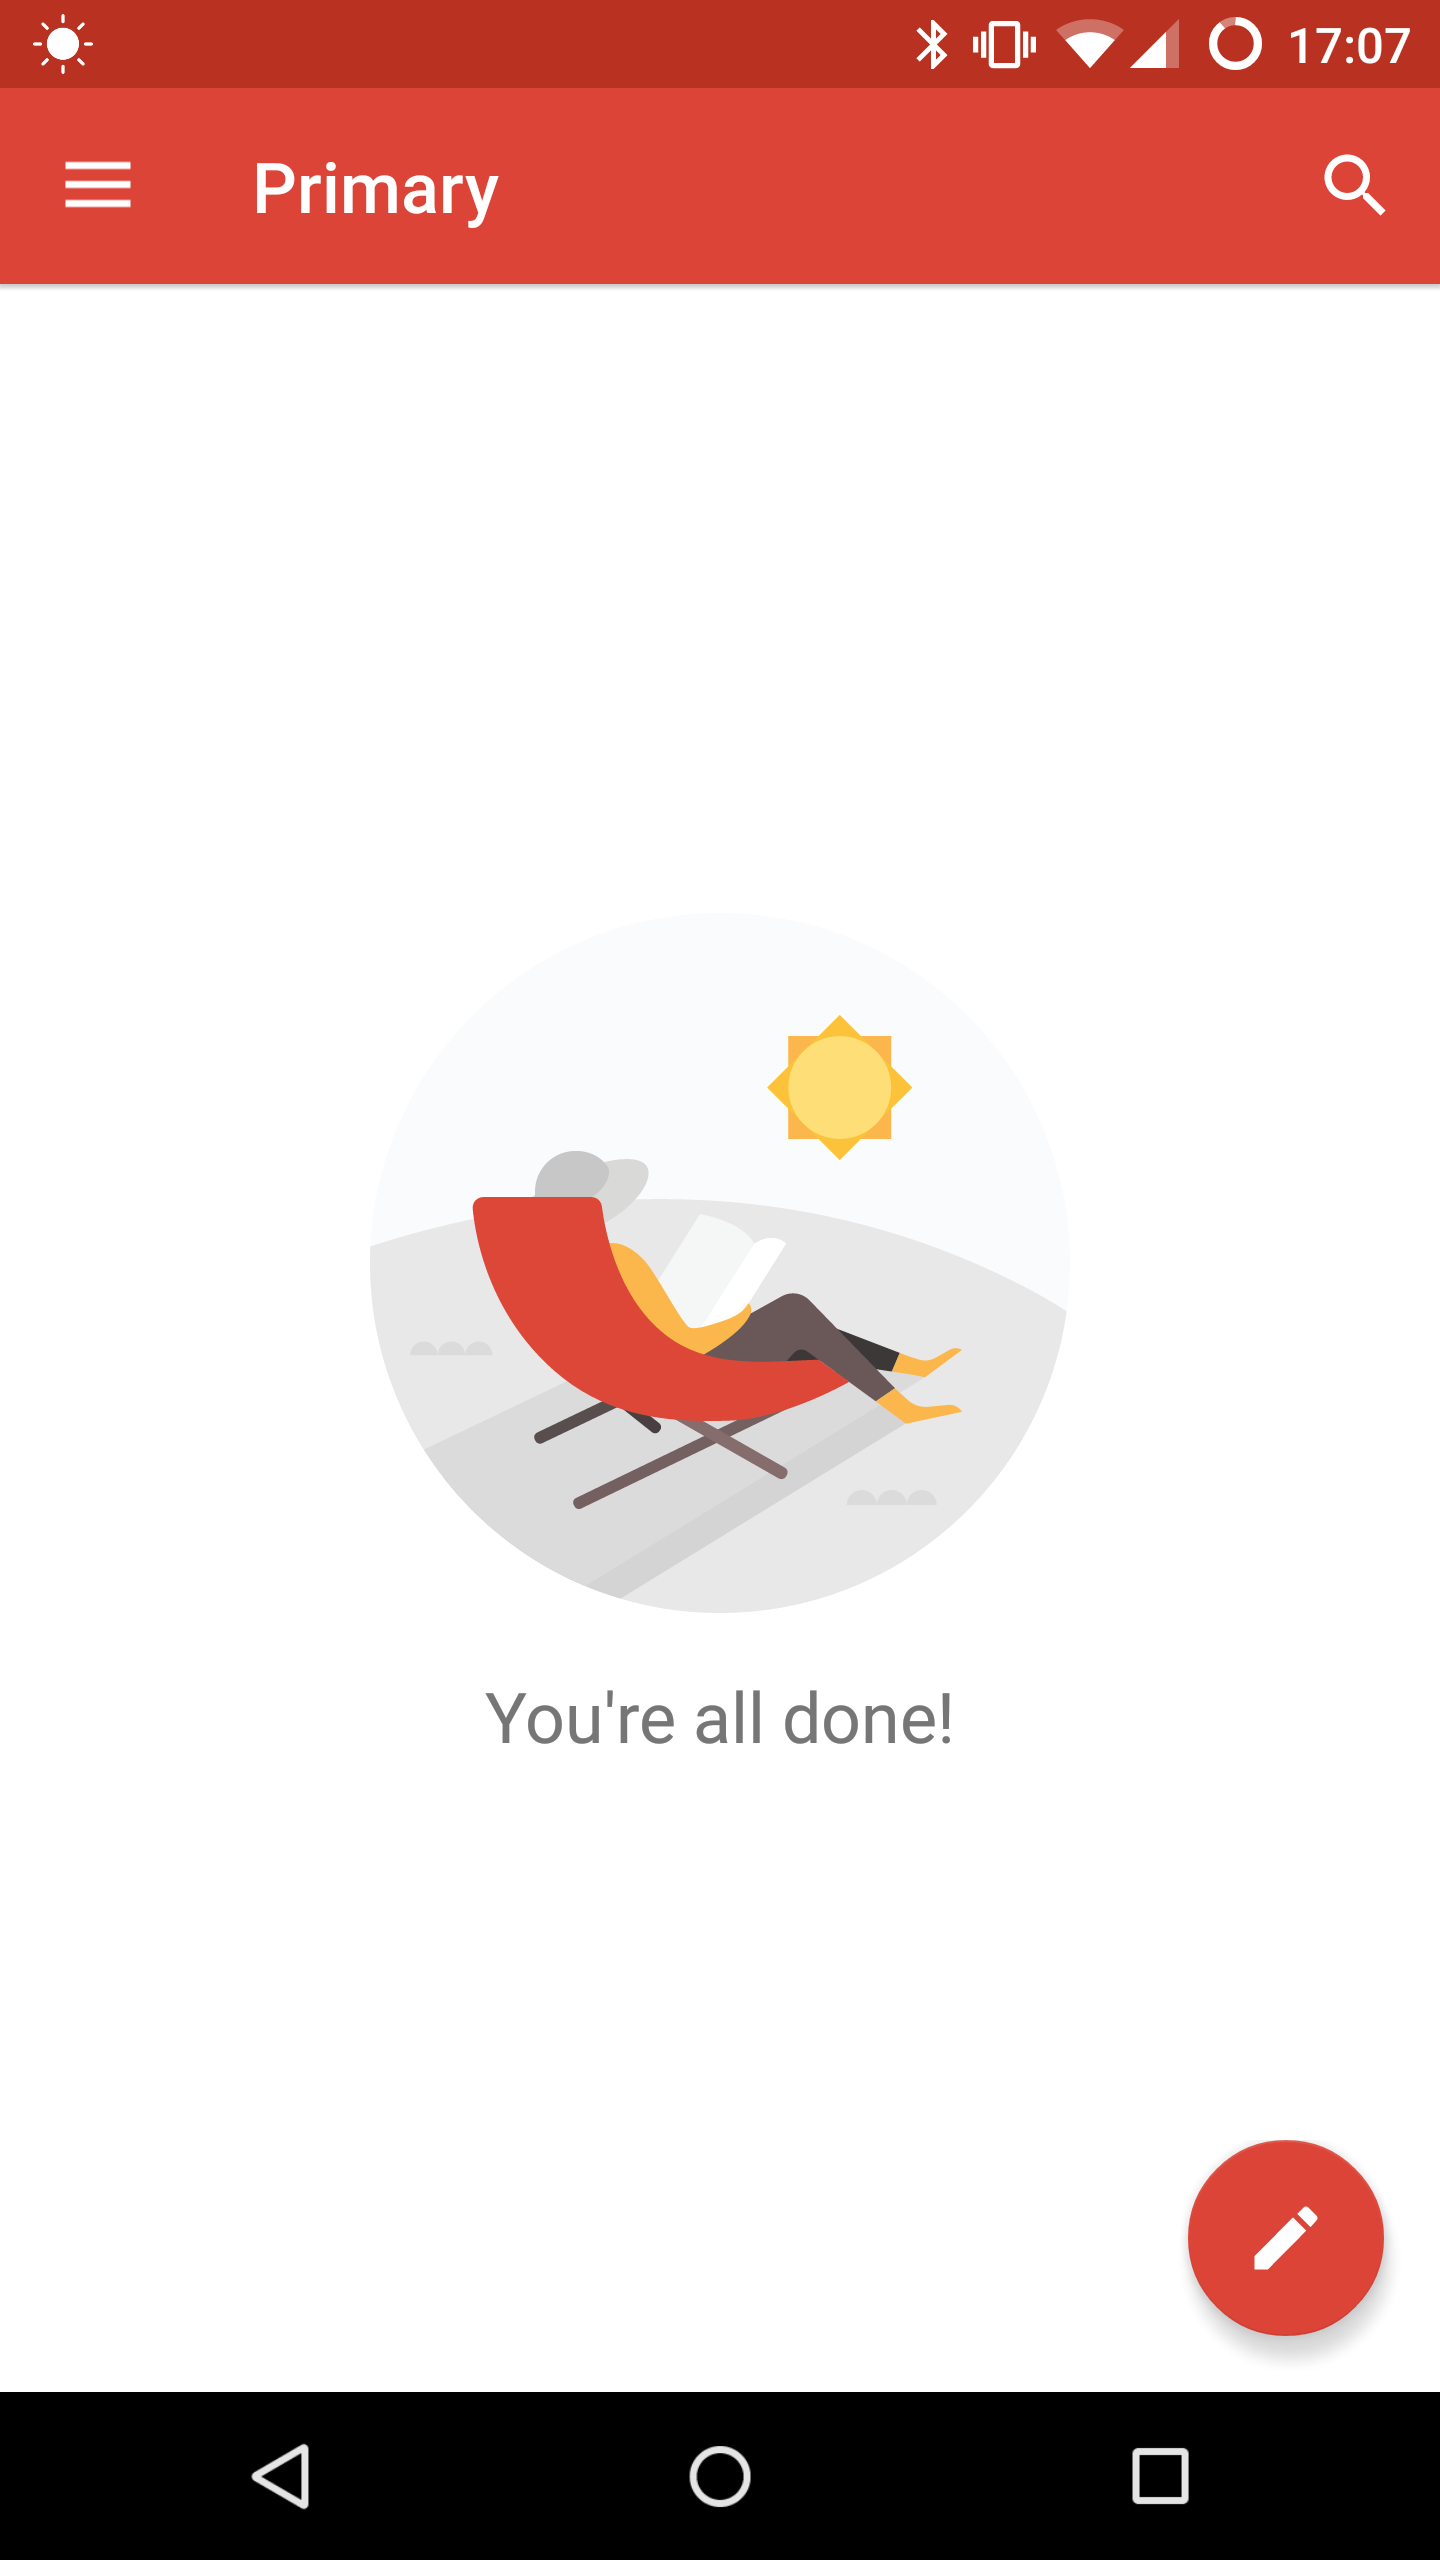
\includegraphics[scale=0.1]{figures/findings/fab-Gmail.png} }}%
	\qquad
	{{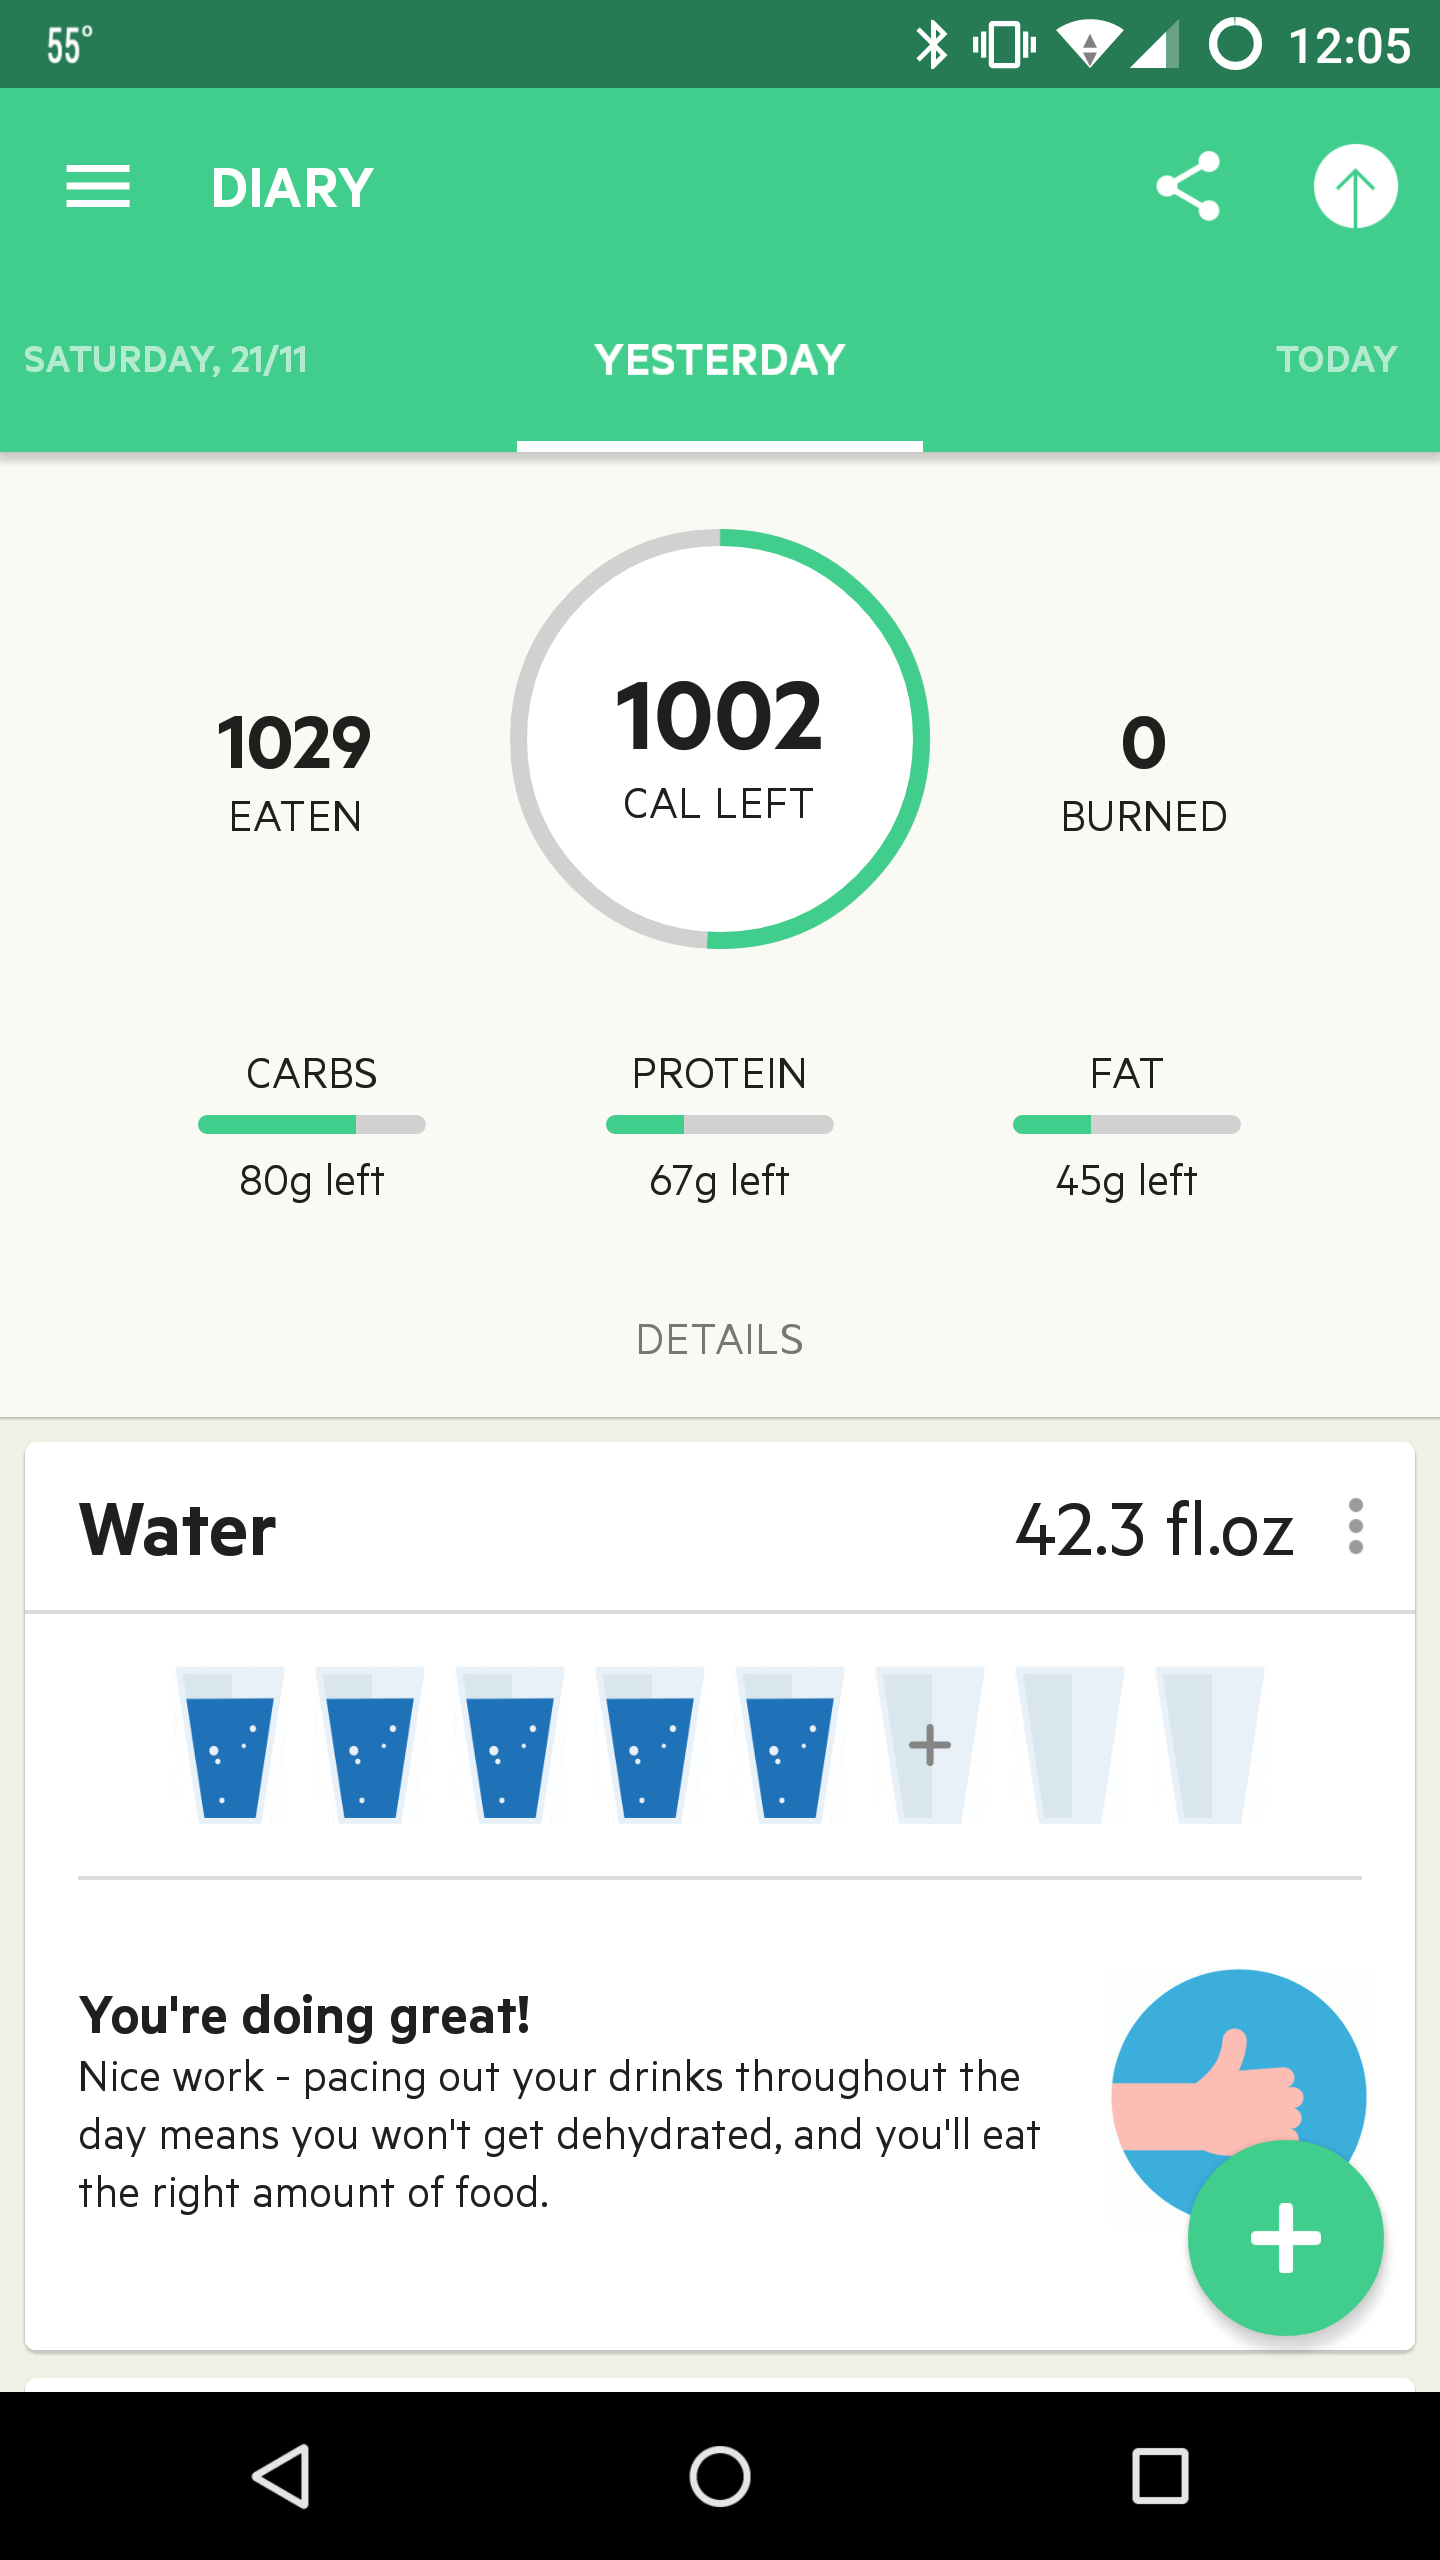
\includegraphics[scale=0.1]{figures/findings/fab-lifesum.png} }}%
	\caption{The Floating Action Button (FAB) shown at the bottom right corner of two apps, Gmail and Lifesum}%
	\label{fig:figure_fab_screenshot}
\end{figure}
The Floating Action Button (FAB) is a circled button floating above the UI to promote the primary action in the app (Figure~\ref{fig:figure_fab_screenshot}).
While developers can create a custom FAB with material design style, there are a few libraries that simplify adding this widget.
We can use Sieveable to aid developers and make an informed decision of using a specific library over other alternatives.
With Sieveable, one can examine the popularity of a specific UI library within any time window.
This can provide insightful feedback to UI framework engineers or developers on how well the components they developed are received by third-party developers.
We can find the trends of adopting the FAB as a design pattern over time using different alternatives.
At the time of writing, there are four alternative ways to implement the FAB in Android: the official design support library \cite{Android_Design_Support_Lib}, and three other additional third-party libraries \cite{android-floating-action-button, FloatingActionButton, fab}.
I use the following Sieveable search queries to retrieve a set of apps that implement the FAB using the previously mentioned libraries: 

\inputminted
[
framesep=2mm,
baselinestretch=1.2,
bgcolor=MyLightGrayColor,
fontsize=\footnotesize
]
{xml}{figures/source-code/fab.txt}

\noindent When we combine all the results together and aggregate by the release year in which the first adoption is observed, we can get a sense of the adoption rate of the FAB over the last years as shown in figure~\ref{fig:fab_years}.
\begin{figure}[h]
	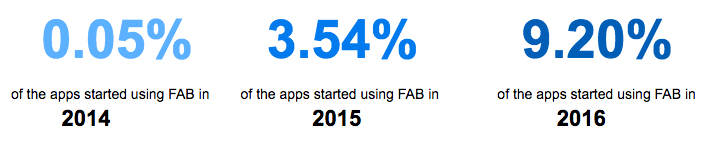
\includegraphics[scale=0.6]{figures/findings/fab_over_years.png}
	\caption{The adoption rate of the Floating Action Button (FAB) over the years.}
	\label{fig:fab_years}
\end{figure}
This shows that the adoption rate of this design pattern is growing slowly since it was first introduced in June 2014.
We can also analyze the adoption rate of the different implementation or library options over time.
\begin{figure}[h]
	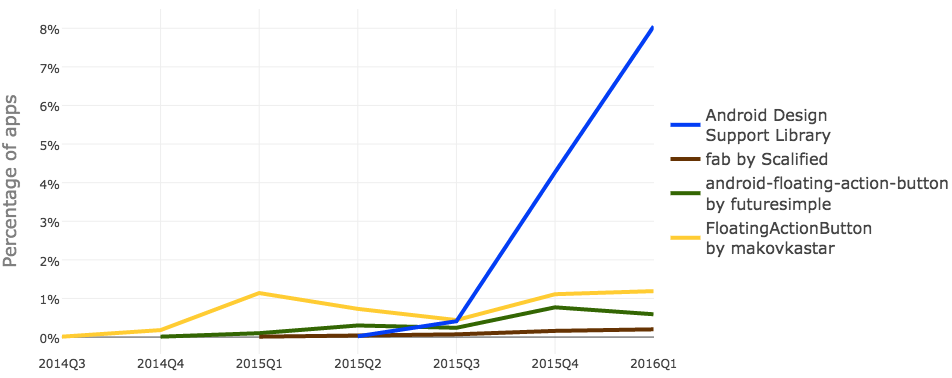
\includegraphics[scale=0.5]{figures/findings/fab_by_quarter.png}
		\caption{The percentage of apps that started adopting the Floating Action Button (FAB) using four popular libraries by calendar quarter.}
	\label{fig:fab_by_quartert}
\end{figure}
In Figure~\ref{fig:fab_by_quartert}, we can see that apps started adopted this pattern before the official release.
Once the official library was introduced by Google in May 2015 \cite{android_design_support_lib_blog_post}, the adoption rate started to increase noticeably.
This shows that a small number developers tend to use third-party libraries to implement a new design that is not yet officially supported.
The larger number of developers, however, are much quicker to use a consistent implementation by an official library.
Finally, I analyzed the group of apps that started adding FAB earlier using a third-party library before the existence of the official library.
I found that the majority of these apps have a low number of downloads (89.81\% with 100,000 download times or less compared to 10.19\% with more than 100,000 download times).

\subsubsection{Navigation Drawer}
\begin{figure}[H]
	\centering
	{{
\includegraphics[scale=0.1]{figures/findings/closed-nav-drawer-kitchenstories.png} }}%
	\qquad
	{{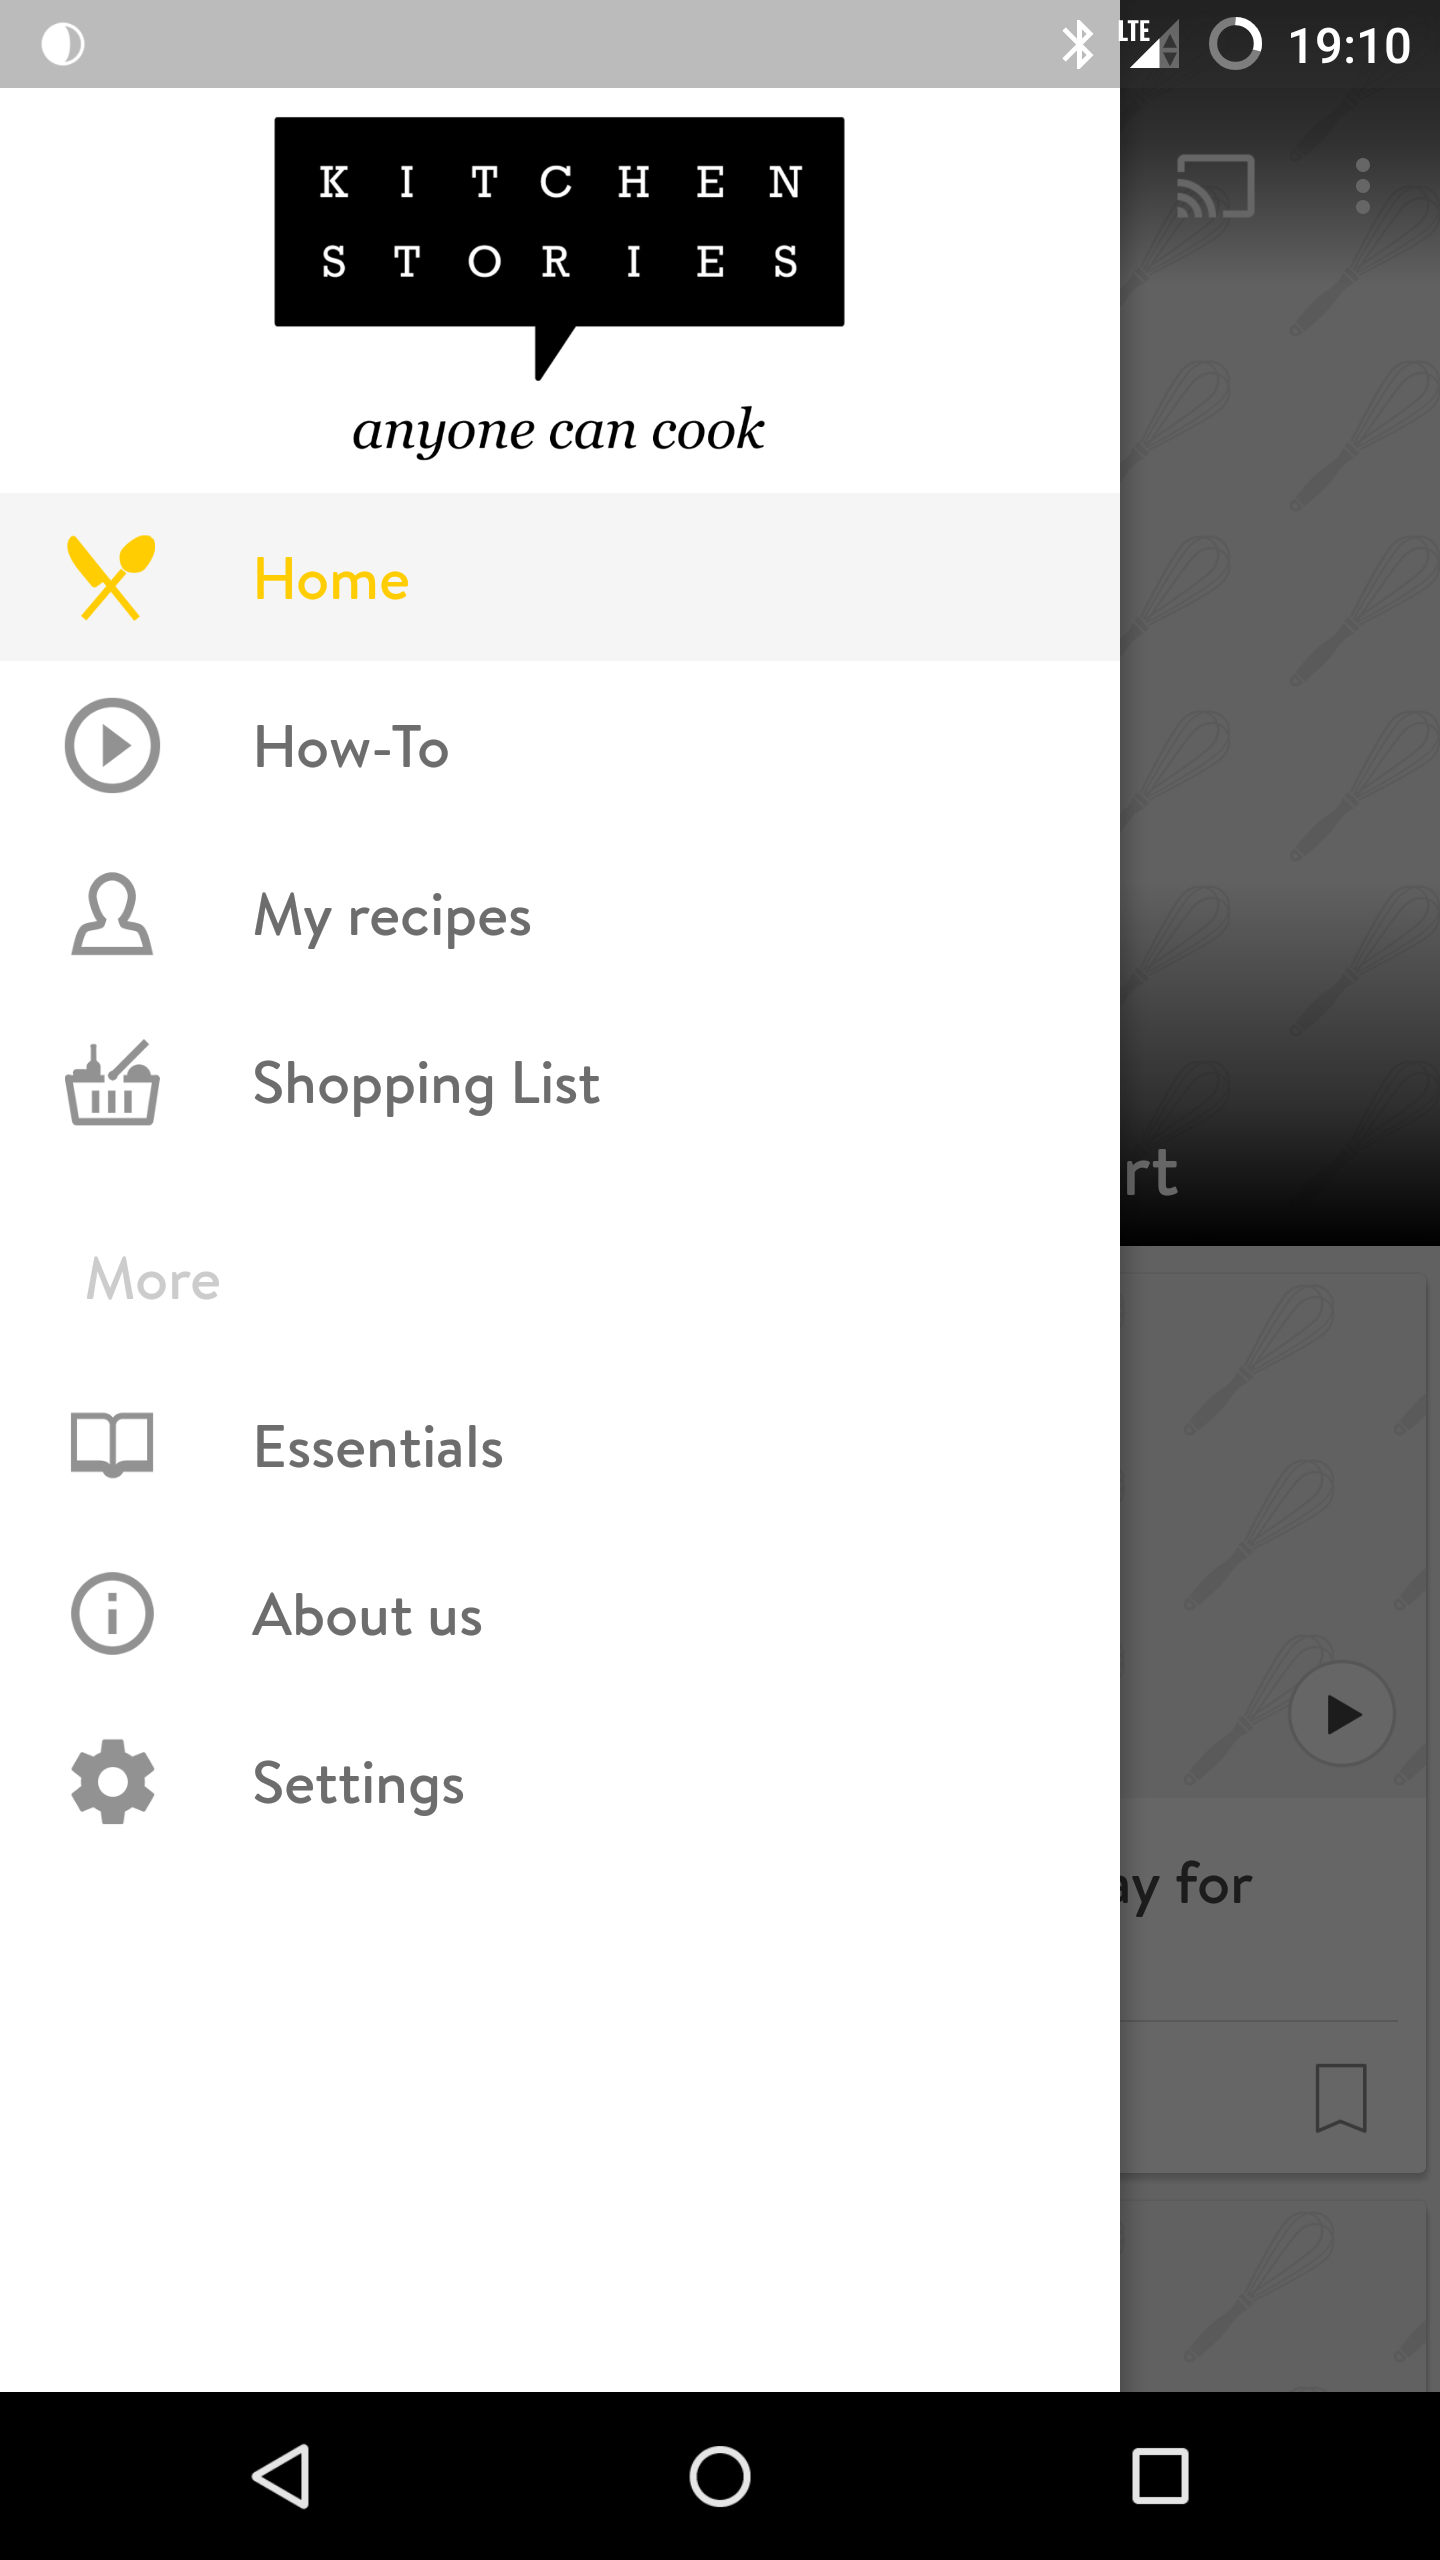
\includegraphics[scale=0.1]{figures/findings/open-nav-drawer-kitchenstories.png} }}%
	\caption{Example of an app with a closed navigation drawer (left) and an open navigation drawer (right).}
	\label{fig:nav_drawer}
\end{figure}
The navigation drawer is a hidden menu panel that can be revealed by tapping on the app icon menu (also known as the hamburger icon), which causes the panel to slide from left to right (figure~\ref{fig:nav_drawer}).
The navigation drawer has existed before the concepts of material design were introduced and was later added to the list of material design patterns with minor styling recommendation.
In order to create a navigation drawer, a developer needs to add a root element to the layout file with two children.
The root element must be a specific view called \textit{android.support.v4.widget.DrawerLayout}, which holds two children.
The first child can be any view group element to hold the content of the app.
The second child is a view that contains the content of the navigation drawer, which can be populated statically or dynamically with the drawer's list of items (e.g., \textit{ ListView} or \textit{android.support.design.widget.NavigationView}).
To find apps with a navigation drawer, I use the following Sieveable search queries:

\inputminted
[
framesep=2mm,
baselinestretch=1.2,
bgcolor=MyLightGrayColor,
fontsize=\footnotesize
]
{xml}{figures/source-code/navdrawer.txt}

\noindent These two search queries returned 20,165 unique apps in total.
To find the adoption rate of this design pattern over the years, I remove duplicate apps from the results, keep the first version in which the adoption is observed, and group the remaining results by year.
Below, figure~\ref{fig:navdrawer_years} shows the adoption rate of the navigation drawer over the years from 2013 to 2016.
We can see an increase over the years but at a relatively slow rate (6.95\% is the average annual adoption increase).
\begin{figure}[h]
	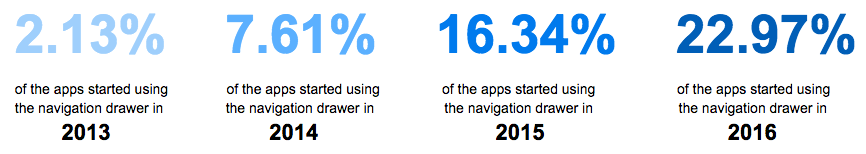
\includegraphics[scale=0.55]{figures/findings/navdrawer_over_years.png}
	\caption{The adoption rate of the Navigation Drawer over the years.}
	\label{fig:navdrawer_years}
\end{figure}
We can group the results by the release date quarterly and download count to see the trends in adopting this design pattern among most and less downloaded apps.
To better approximate the popularity of Android apps, I group the apps by download count into three main groups: a) most downloaded apps for apps with one million or more download times, b) middle downloaded apps for apps with 100,000 and fewer than 1,000,000 download counts, and c) least download apps for apps with fewer than 100,000 download counts.
Figure~\ref{fig:navdrawer_quarter_download} shows that the adoption rate of the navigation drawer is more prevalent in apps with the most download count than others with the exception of the first two quarters of 2015.
\begin{figure}[h]
	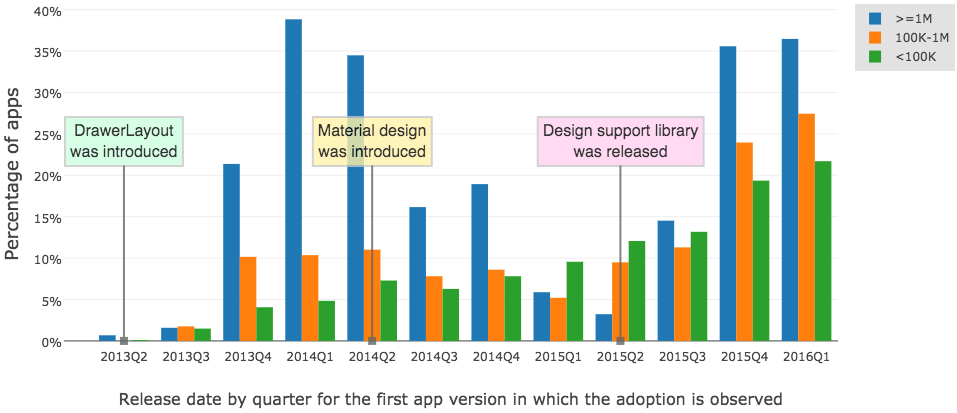
\includegraphics[scale=0.5]{figures/findings/navdrawer_by_quarter_grouped_by_downloads.png}
	\caption{The percentage of apps that started adopting the navigation drawer grouped by three download count groups: most, middle, and least downloaded apps. The x axis shows the calendar quarter of the release date in which the adoption is observed, and the y axis shows the percentage of apps that adopted it. The percentage value is computed by dividing the number of adopted apps in each quarter over the total of apps released in each quarter. The time of major platform events is also marked in the chart.}
	\label{fig:navdrawer_quarter_download}
\end{figure}

\section{Accessibility Mining Analysis}

\section{Security Mining Analysis}
